\documentclass{article}
\usepackage{tikz}
\usetikzlibrary{automata,positioning}

\begin{document}

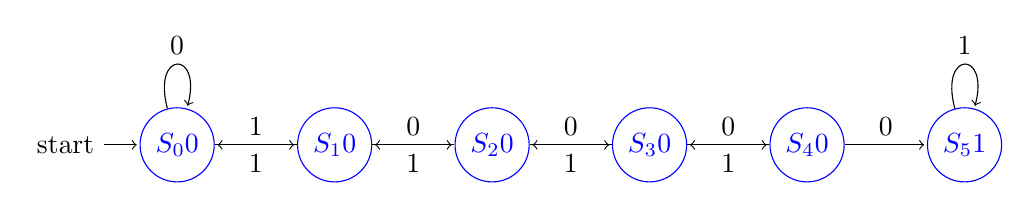
\begin{tikzpicture}[shorten >=1pt,node distance=2cm,on grid,auto]
    \node[state,initial,blue] (q_0) {$S_0$ \\ $0$};
    \node[state,blue] (q_1) [right=of q_0] {$S_1$ \\ $0$};
    \node[state,blue] (q_2) [right=of q_1] {$S_2$ \\ $0$};
    \node[state,blue] (q_3) [right=of q_2] {$S_3$ \\ $0$};
    \node[state,blue] (q_4) [right=of q_3] {$S_4$ \\ $0$};
    \node[state,blue] (q_5) [right=of q_4] {$S_5$ \\ $1$};

    \path[->]
        (q_0) edge [loop above] node {0} ()
              edge node {1} (q_1)
        (q_1) edge node {0} (q_2)
              edge node {1} (q_0)
        (q_2) edge node {0} (q_3)
              edge node {1} (q_1)
        (q_3) edge node {0} (q_4)
              edge node {1} (q_2)
        (q_4) edge node {0} (q_5)
              edge node {1} (q_3)
        (q_5) edge [loop above] node {1} ();
\end{tikzpicture}

\end{document}